\documentclass[conference,a4paper]{IEEEtran}
\IEEEoverridecommandlockouts

\usepackage[hidelinks]{hyperref}
\usepackage[cmex10]{amsmath}%American Math Society(AMS) math formatting
\usepackage{amssymb,amsfonts}%AMS extra symbols and fonts
\interdisplaylinepenalty=2500%allow line breaks in multi-line formulas
\usepackage{dblfloatfix}%fix double column figure ordering and placement

\usepackage[ruled,vlined]{algorithm2e}
\usepackage{graphicx}
\graphicspath{{Figures/PDF/}{Figures/PNG/}}

\usepackage{booktabs}
\usepackage{siunitx}
\usepackage[numbers,compress]{natbib}
\usepackage{texnames}
\usepackage{bm,bbm}
\usepackage{orcidlink}

\begin{document}

\title{\uppercase{\LaTeX\ Template for IGARSS 2025 Articles (with \BibTeX)}
\thanks{Identify applicable funding agency here. If none, delete this.}
}

\author{	\IEEEauthorblockN{Alejandro C.\ Frery\orcidlink{0000-0002-8002-5341}}
	\IEEEauthorblockA{\textit{Victoria University of Wellington}\\
		6140 Wellington, New Zealand\\
		alejandro.frery@vuw.ac.nz}
	\and
	\IEEEauthorblockN{Hui Zhang\orcidlink{0000-0002-5283-7350}}
	\IEEEauthorblockA{\textit{Inner Mongolia University}\\
		010021 Hohhot, China\\
		hui.zhang@imu.edu.cn}
	\and
	\IEEEauthorblockN{Andrea Rey\orcidlink{0000-0002-9185-1382}}
	\IEEEauthorblockA{\textit{Universidad Nacional de Hurlingham}\\
		1688 República Argentina\\
		andrea.rey@unahur.edu.ar}
}


\maketitle
%\begin{abstract}
%	If this were an actual abstract, I would state the research question and why it is relevant for the community that will attend IGARSS2025. I'd boldly say that this has not been done before in the way I've done it. Then, I would give an idea of the approach I took and summarize my key findings. I would conclude the abstract by stating how these findings serve to answer my research question.
%\end{abstract}
\begin{abstract} This paper proposes a computationally efficient algorithm to address the Full-Waveform Inversion (FWI) problem with a Total Variation (TV) constraint, designed to accurately reconstruct subsurface properties from seismic data.
FWI, as an ill-posed inverse problem, requires effective regularizations or constraints to ensure accurate and stable solutions.
Among these, the TV constraint is widely known as a powerful prior for modeling the piecewise smooth structure of subsurface properties.
However, solving the optimization problem is challenging because of the nonlinear observation process combined with the non-smoothness of the TV constraint.
Conventional methods rely on inner loops and/or approximations, which lead to high computational cost and/or inappropriate solutions.
To address these limitations, we develop a novel algorithm based on a primal-dual splitting method, achieving computational efficiency by eliminating inner loops and ensuring high accuracy by avoiding approximations.
We also demonstrate the effectiveness of the proposed method through experiments using the SEG/EAGE Salt and Overthrust Models.
 \end{abstract}

\begin{IEEEkeywords}
	IGARSS 2025, \LaTeX, reproducibility, template.
\end{IEEEkeywords}


\section{Introduction}

This template is aligned with the good practices stated by \citet{EditorialGRSL2015}, which are a step towards a reproducible article \citep{ABadgingSystemforReproducibilityandReplicabilityinRemoteSensingResearch}.
We used the official IEEE Conference Proceedings template available here \url{https://www.ieee.org/conferences/publishing/templates.html} to produce this simplified version for IGARSS~2025.
This template uses \BibTeX, a convenient way of managing references that simplifies the formatting and automatically selects the bibliographic entries cited in the text.

A basic knowledge of \LaTeX\ and \BibTeX\ is required.

\section{Document Structure}

Conceptually, a scientific document should have four elements:
\begin{itemize}
	\item Introduction: your scientific question, the review of the literature, an outline of the steps you took to answer, a summary of what you observed, and a brief statement of how those observations changed the state-of-the-art (that was outlined in the review of the literature).
	\item Methodology: describe what you did so other researchers can replicate your study.
	\item Results: the core observations you collected, usually summarized in tables, figures, and images.
	\item Discussion: this is the essential part of your work. Do not summarize your results. Tell the reader how they answer (or not) your scientific question and how they change the state-of-the-art.
\end{itemize}
This structure is known as ``IMRaD,'' and was consolidated by over a century of scientific practice.
Fig.~\ref{fig:IMRAD} shows a quote from the book by \citet{Day1998} about this structure, and this piece of code shows how to include a figure in your article.
The file is in PNG format; reserve this format for matrix-like graphical elements.
Use PDF for plots, as in Fig.~\ref{fig:Densities}.

\begin{figure}[hbt]
	\centering
	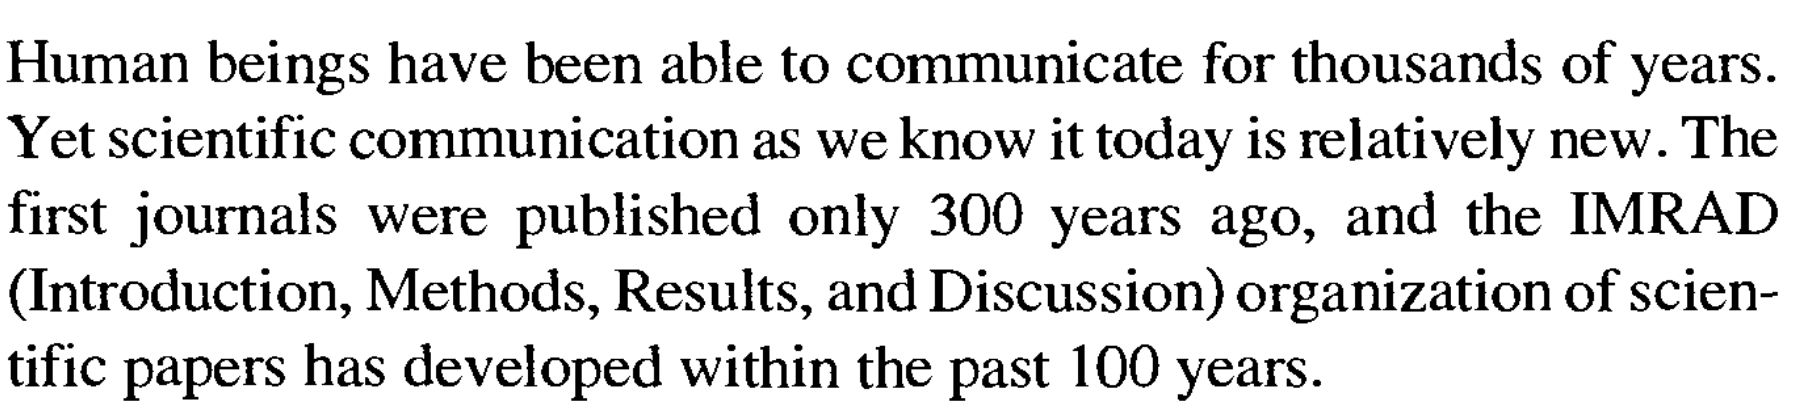
\includegraphics[width=.9\linewidth]{Day-IMRaD}
	\caption{A screenshot from \citet{Day1998} about the structure of a scientific article.}\label{fig:IMRAD}
\end{figure}

The main textual components are controlled by the commands \verb|\section|, \verb|\subsection|, and \verb|\subsubsection|.

\subsection{This is a subsection}

Text components are automatically numbered.

\subsubsection{This is a subsection inside a subsection} This is the innermost text component you should use in your document. 
It appears as a paragraph with a title.

\subsubsection{Nice tables} Citing \citet{simplexCT}:
\begin{quote}
	Tables are best suited for looking up precise values, comparing individual values or presenting values involving multiple units of measure. Graphs, on the other hand, are better for detecting trends, anomalies or relations. In other words, graphs show the forest while tables show the trees.
\end{quote}

Once you have designed your table, type it using commands from \verb|booktabs|, as in Table~\ref{tab:MyTable}.
Notice that the second column type was stipulated with commands from the \verb|siunitx| package.
It switches to mathematical mode and aligns the figures by their decimal point, promoting an immediate visual comparison.

\begin{table}[hbt]
	\centering
	\caption{True and estimated classes, with the sample mean.}\label{tab:MyTable}
	\begin{tabular}{r S[table-format=3.2] l}
		\toprule
		\textbf{True LULC} & \textbf{Mean} & \textbf{Estimated LULC} \\ \cmidrule(lr){1-1} \cmidrule(lr){2-2}\cmidrule(lr){3-3}
		Sand & 1.32 & Open sea\\
		Forest & 7.93 & Forest\\
		Open sea & -5 & Open sea\\
		Bare soil & 100.41 & Bare soil\\ \bottomrule
	\end{tabular}
\end{table}

Tables and algorithms captions are usually at the top,
while figures captions are at the bottom.

\subsection{Another subsection}

Your document should have at least two components for each level, i.e., do not use a single \verb|\subsubsection|, but at least two.

One of \LaTeX's strongest abilities is producing high-quality equations:
\begin{equation}
	i\hbar \frac{\partial}{\partial t} \Psi(\bm{r}, t) = \widehat{H} \Psi(\bm{r}, t),
\end{equation}
where $i=\sqrt{-1}$ is the imaginary unit,
$\hbar$ is the reduced Plank's constant,
${\partial}/{\partial t}$ is the partial derivative operator with respect to time,
$\Psi(\bm{r}, t)$ is the wave equation that depends on the position $\bm r$ and time $t$, and
$\widehat{H}$ is the Hamiltonian operator.
Always detail every component of each equation.

Use \verb|amsmath|'s mathematical environments:
\begin{equation}
	f_{\text{tr} A}(x) =
	\Big| \frac{x\beta}{2} \Sigma^{-1} \Big|^a
	\frac{e^{-z}}{x\Gamma(ma)} {}_1F_x^{(2a)} 
	\Big(a;ma;z I_m - \frac{x\beta}{2}\Sigma^{-1}\Big),
\end{equation}
in which we have followed the notation defined by \citet{TheDensitiesandDistributionsoftheLargestEigenvalueandtheTraceofaBetaWishartMatrix}.
The package offers several options to align equations.
Often, an equation is wider than a column; in that case, use the \verb|\begin{multline} ... \end{multline}| environment.
\begin{multline}
	\Pr\big(\text{tr} A \leq (x)\big) =
	\Big| \frac{x\beta}{2} \Sigma^{-1} \Big|^a
	\frac{1}{\Gamma(ma+1)} \\ 
	{}_1F_x^{(2a)} \Big(a;ma+1;- \frac{x\beta}{2}\Sigma^{-1}\Big).
\end{multline}

\subsection{Algorithms}

Algorithms summarize, in readable form, the steps that comprise a computational procedure.
Algorithm~\ref{algo:TwoColumns} shows an example using the \verb|algorithm2e| package.
This pseudocode spans two columns.

\begin{algorithm*}[hbt]
	\DontPrintSemicolon
	\SetKwInput{KwCompute}{Compute}
	\SetKwInput{KwDefine}{Define}
	\caption{Quasi $U$-Statistics}\label{algo:TwoColumns}
	\KwData{The list of folders $\mathcal L$}
	\KwData{The number of groups $G$.}
	\KwData{The sample size per group $n_1,n_2,\dots,n_G$.}
	\KwData{The data per group $\bm X_{1},\ldots,\bm X_{n_1},\bm X_{n_1+1},\ldots,\bm X_{n-n_G+1},\ldots,\bm X_{n_G}$.}
	\KwData{The number of bootstrap replications $B$ (we used $200$).}
	\KwCompute{Choose the kernel $\phi$ of degree two from 
		\begin{align*}
			\phi_1(x,y)&=|x-y|^p,\\
			\phi_2(x,y)&=\mathbbm{1}\left\{|x-y|>\eta\right\}.
	\end{align*}}
	\KwCompute{Select $p$ for $\phi_1$, or $\eta$ for $\phi_2$, e.g., with a data-drive optimization method.}
	\KwDefine{Define $T$ as
		\[
		T=\sum\eta_{nij}\phi(\bm X_i,\bm X_j),
		\]
		where the weights are given by:
		\[
		\eta_{nij}=\begin{cases}
			1 & \text{if } i \text{ and } j \text{ belong to different groups,}\\
			-\frac{(n-n_g)}{(n_g-1)} & \text{if } i \text{ and } j \text{ belong to group } g, \text{ for each } 1\leq g\leq G.
		\end{cases}
		\]}
	\While{$\mathcal L$ has elements}{
		Read the following element $\ell$ in the list $\mathcal L$\;
		\If{$\ell$ is empty}{Skip to the next element\;}
		\Else{
			\KwCompute{Compute $T$ on the sample $\bm X_{1},\ldots,\bm X_{n_1},\bm X_{n_1+1},\ldots,\bm X_{n-n_G+1},\ldots,\bm X_{n_G}$ and store it in $T_{\text{obs}}$}
			\For{$1\leq b \leq B$}{
				Build the bootstrap sample $\bm X^{(b)}=\big(\bm X_{1}^{(b)},\ldots,\bm X_{n_1}^{(b)},\ldots,\bm X_{n-n_G+1}^{(b)},\ldots,\bm X_{n_G}^{(b)}\big)$\;
				Compute $T^{(b)}$ with $\bm X^{(b)}$
			}
			Compute $q_\alpha$, the upper $\alpha$ quantile of $T^{(1)},T^{(2)},\dots, T^{(B)}$\;
			\KwOut{Decision: reject $H_0$ if $T_{\text{obs}}>q_\alpha$.}
			Remove the current set from the list $\mathcal L$\;
		}
	}
\end{algorithm*}

\subsection{Units}

It is mandatory to state the measurement units.
The \verb|siunitx| provides commands that implement some of the best ways to do it.
For instance, you type \verb|\SI{10}{\mega\hertz}| and produce \SI{10}{\mega\hertz}.
You type \verb|\qtyproduct{2x5}{\meter}| and produce \qtyproduct{2x5}{\meter}, e.g., for stating the spatial resolution of an image.

\section{Figures}

Fig.~\ref{fig:Densities} shows a PDF figure.
Notice that the font size is readable in the final version.

\begin{figure}[hbt]
	\centering
	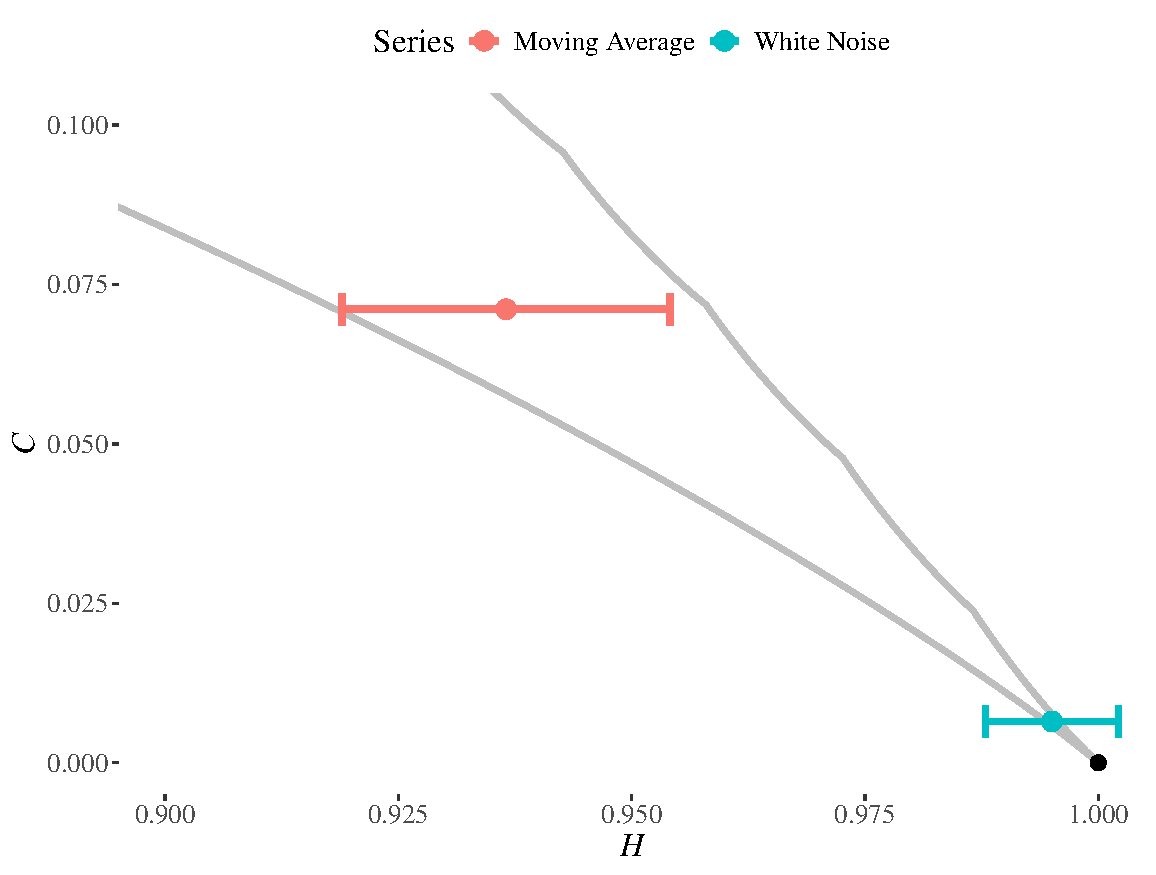
\includegraphics[width=\linewidth]{SinglePlot}
	\caption{Two time series mapped onto their Shannon Entropy ($H$) and Statistical Complexity ($C$) points along with \SI{95}{\percent} confidence intervals for the entropy using $D=4$ embedding dimension; cf.\ \citet{AsymptoticDistributionofEntropiesandFisherInformationMeasureofOrdinalPatternswithApplicationsa}.}\label{fig:Densities}
\end{figure}

Making reproducible plots and storing the code that produced them is more than advisable.
The plot displayed in Fig.~\ref{fig:Densities} was created with R~\cite{AmazingR}, and the code is in the \verb|Code| folder accompanying this template.
It requires a few packages: \verb|ggplot2|~\citep{ggplot2}, \verb|ggthemes|~\citep{ggthemes}, and
\verb|StatOrdPattHxC|~\citep{AsymptoticDistributionofEntropiesandFisherInformationMeasureofOrdinalPatternswithApplicationsa}.

Notice that I used \verb|theme_tufte()| to obtain a minimalistic yet informative plot.
I recommend the books by E.\ Tufte~\citep{Tufte01,VisualExplanationsImagesandQuantitiesEvidenceandNarrative,EnvisioningInformation,BeautifulEvidence} are my preferred reference for communicating with graphics.

\section{References using \BibTeX}

This template shows how to use \BibTeX.
The \texttt{natbib} package allows several types of citations.
Notice the convenience of using \verb|\citet|, as in the book by \citet{BrockwellDavis91}.
There is also the \verb|\citep| option, where the reference is inserted between parenthesis \citep{OverviewofthePolSARproV4.0SoftwaretheOpenSourceToolboxforPolarimetricandInterferometricPolarimetricSARDataProcessing}.
The \verb|references.bib| file provides examples of a journal article~\citep{ABadgingSystemforReproducibilityandReplicabilityinRemoteSensingResearch},
a technical report~\citep{SystemCalibrationStrategiesforSpaceborneSyntheticApertureRadarforOceanography}, a conference article~\cite{OverviewofthePolSARproV4.0SoftwaretheOpenSourceToolboxforPolarimetricandInterferometricPolarimetricSARDataProcessing}, a book~\cite{BrockwellDavis91}, a manual~\cite{ERMANIIUsersManual}, and a website~\cite{simplexCT}.

\small
\bibliographystyle{IEEEtranN}
\bibliography{references}

\end{document}